\documentclass[11pt]{article}
\usepackage{color}
\usepackage{authblk}%allows footnote format for authors
\usepackage[letterpaper, margin=1in]{geometry} %package that allows changes in margins and header/footers
\usepackage{natbib}
\usepackage{amsmath}
\usepackage{rotating}
\usepackage{adjustbox}
\usepackage[english]{babel}
\usepackage{colortbl}
\usepackage{booktabs}
\usepackage{tabularx}
\usepackage[x11names,dvipsnames,table]{xcolor}
\usepackage{lineno}
\linenumbers
\usepackage{array}
\bibliographystyle{GenRes.bst}
\renewcommand{\baselinestretch}{1.5}
\newcommand{\mbh}[1]{\textcolor{red}{ \emph{\scriptsize  #1}} } %creating command for Matt's comments
\newcommand{\esw}[1]{\textcolor{blue}{ \emph{\scriptsize  #1}} } %creating command for Matt's comments

\title{Evidence-driven Annotation of Plant Genome Assemblies}

\author[1]{Authors: Arun S. Seetharam}%author information
\author[2]{Jacqueline Campbell}
\author[2]{Sagnik Banerjee}
\author[2]{Margaret Woodhouse}
\author[2]{Carson Andorf}
\author[2]{Ethalinda Cannon}
\author[2]{Steven Cannon}
\author[2]{Eve Wurtele}
\author[3]{Matthew B. Hufford}
\affil[1]{Genome Informatics Facility, Iowa State University, Ames, Iowa 50011, USA}
\affil[2]{Department of Genetics, Development, and Cell Biology, Iowa State University, Ames, Iowa 50011, USA}
\affil[3]{Department of Ecology, Evolution, and Organismal Biology, Iowa State University, Ames, Iowa 50011, USA}
\date{}

\begin{document}

\maketitle

\clearpage

\section*{Summary}

\section*{Introduction}

Below you will see some \textit{syntax} for including a figure in a manuscript.
The file for the figure must be in the same folder as this .tex file.
And LaTeX makes it super easy to cite figures in the manuscript--no need to keep track of figure numbers, just the label associated with them.
For instance, to cite the map below, I just type (Figure \ref{fig:map}).
Please remember to return to a new line when you start a new sentence.
\esw{this is eve's first comment}

New paragraphs can be started by including two returns.
\mbh{And here you can see how I can make a comment in the text}
Isn't LaTeX easy and fun?

\begin{figure}[h]
  \centering
     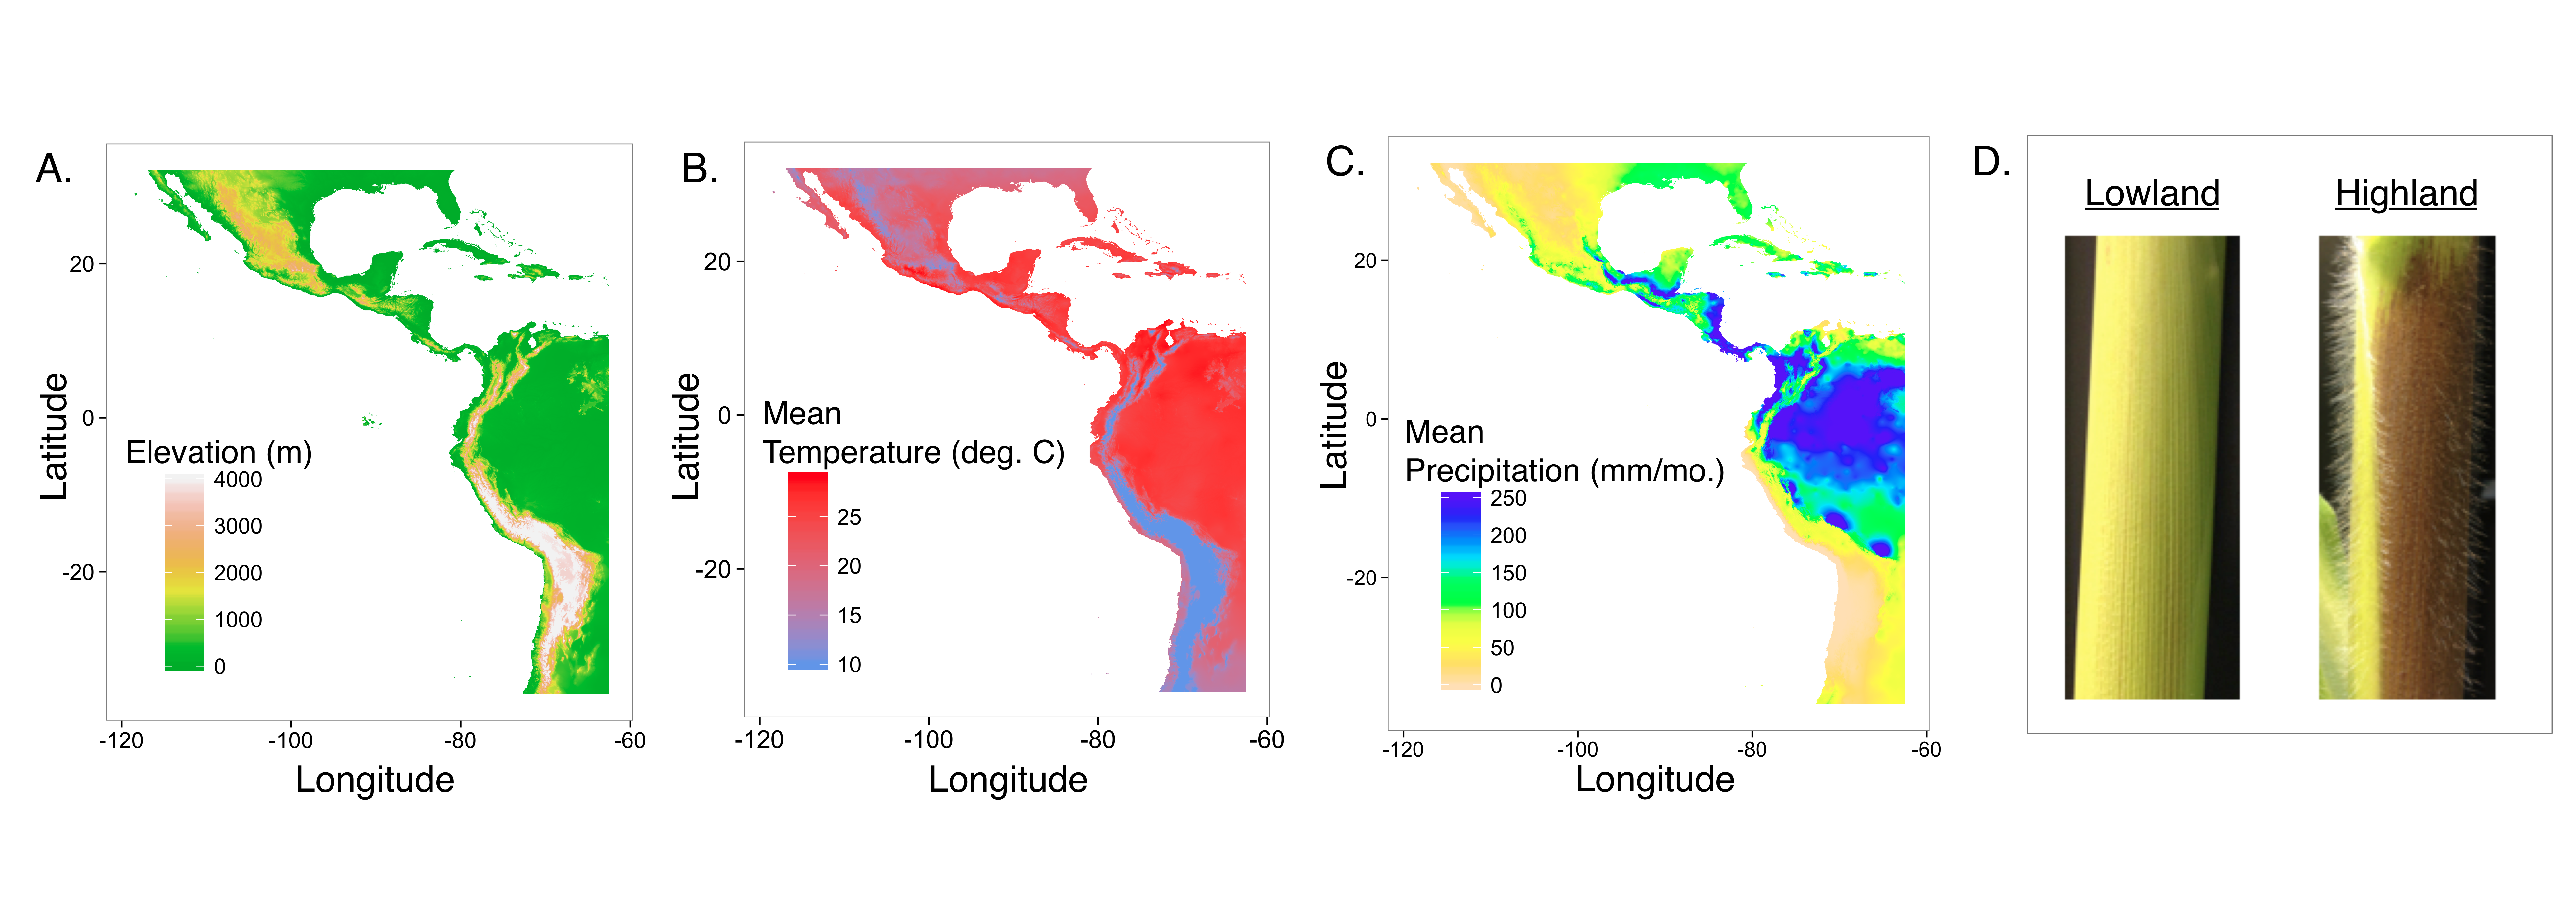
\includegraphics[width=\textwidth]{MapFigure_highres.png}
  \caption{Climate varies considerably across our focal maize habitats of Mexico and western South America. Variables of interest include elevation (A), temperature (B), and precipitation (C). Maize from highland and lowland areas of this region differ considerably in multiple phenotypes such as stem morphology (D).}
   \label{fig:map}
\end{figure}

Tables in LaTeX are also really easy and come out looking great.
Below is an example of a table and we can cite this table using this syntax (Table \ref{tab:qtlpops}).
Citations are also really easy.
For example, if I want to cite one of our papers on independent adaptation of maize to high elevation, I would just do this \citep{Takuno2015}.
New citations in bibtex format can be copied from journal websites and pasted into the "Annotation.bib" file included in this directory.

\begin{table}
\rowcolors{2}{white}{gray!25}
\begin{center}
\caption{Parental lines for QTL Populations} \label{tab:qtlpops}
\begin{tabular}{lllll}
\\\toprule  
\rowcolor{white}
{\bf Population}	& {\bf Parent } &	{\bf Origin (masl)} &  {\bf Inbred } & {\bf Status }\\ \midrule
\rowcolor{gray!25}
Mexico	& Zapalote Chico		& Oaxaca	 (46)	& yes	&  F2:3 \\ 
\rowcolor{gray!25}
	& 	Palomero de Jalisco	& 	Jalisco (2520)	& yes	& \\
S. America	& Pororo	& Bolivia (330)	& yes &  F2 \\ 
\rowcolor{white}
	& Maranon	 & Peru (2820) & no & \\ \bottomrule
\end{tabular}
\end{center}
\end{table} 


\section*{Methods}

\section*{Results}

\section*{Discussion}

\bibliography{Annotation.bib}

\end{document}